\section{Laboratory work implementation}

\subsection{Tasks and Points}

There's a legacy system your new client want to extend (without access to its source code). The existing system allows to get a list of orders made by client's customers and a list of categories. The orders are quite simple - created-at, total, user-id, category-id. And a category isn't complicated as well - id, name, category-id<nullable>. Category is a simple recursive data structure (what means that some categories can have as parent another category, and there can be "root" categories which doesn't have a parent).

Your client wants from you a tool which can generate a new type of report - total per categories (including data from child descending categories).

You've got a simple sketch from the client. 
\begin{figure}[!ht]
	\centering
	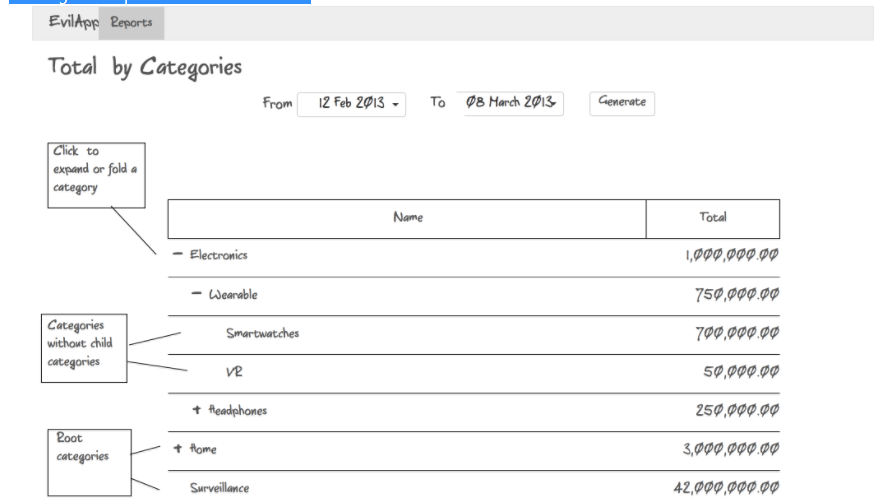
\includegraphics[width=0.4\linewidth]{0}
	\caption{Template de afisare a rezultatelor}
	\label{fig:0}
\end{figure}

There is some info about the legacy system you managed to get from your client:
\begin{itemize}
	\item Categories URL https://evil-legacy-service.herokuapp.com/api/v101/categories/
	\item Orders URL https://evil-legacy-service.herokuapp.com/api/v101/orders/
	\item The client said that he had found a mysterious "key" 55193451-1409-4729-9cd4-7c65d63b8e76 for the legacy system
\end{itemize}
\textbf{Note}: The legacy system isn't documented properly (all you know about it - URL and that it must return CSV), so you need to read about HTTP and discover what additional info you may need to supply to get a response with requested data.
The application must offer next functionality:
\begin{itemize}
	\item retrieve the list of orders (since it's a legacy system, it exports data in CSV format :( ) within a date interval
	\item retrieve the list of available categories (also CSV :( )
	\item parse and validate received data
	\item aggregate data
	\item  display results to the user
	\item cache received data locally
\end{itemize}

\subsection{Analiza lucrarii de laborator}

Pentru realiarea task-urilor descriseanterior a fost folosit limbajul Java. Astfel, programul realizat conține următoarele clase:

\textit{Request} - această clasă are 3 parametri: url(de tip string), key(de tip string) și list(de tip ArrayList). Această clasă are o funcție principală, și anume  getData(). Cu ajutorul parametrilor url și key este realizat reuest-ul, iar datele obținute(în format CSV) sunt salvate și returnate prin parametrul list.(Listing 1)

\textit{Orders} - această clasă are 4 parametri id(int), total(double), category-id(int)
, created(string). Datele obținute în urma request-ului sunt parsate și transformate în obiecte de tip Orders. Funcția de parsare este prezentată în Listing 2.

\textit{Categories} - această clasă are 3 parametri id(int), category-id(int), name(string). Funcționalitatea acesteia este asemănătoare cu cea a clasei Orders, doar că structura obiectelor este diferită.

\textit{ReadOrders} - pentru a crea request-ul și parsarea comenzilor și categoriilor, acestea au fost plasate în 2 fire de execuție diferite, dirijate de un alt fir de execuție. Pentru a crea aceste fire a fost implementată interfața Callable.

\textit{ThreadAgregation} - acestă clasă reprezintă la rândul ei un alt fir de execuție, care va porni simultan cele 2 fire de execuție, reîntorcând controlul thread-ului principal abia după ce ambele fire își vor fi terminat execuția. Implementarea aceasta este prezentată în Listing 3

\textit{Tree} - Cu ajutorul acestei clase a fost implementată afișarea în cascadă. Astfel, fiecare nod creat devine root pentru un nou tree, pină când nodurile nu mai copii. Funcția de afișare este prezentată în Listing 4

În urma implementărilor realizate, rezultatele obținute pot fi vizualizate în figura 1.2.
\subsection{Imagini}

\lstinputlisting[style=mystyle, language=Java, caption={Funcția ce realizează request-ul}, label=paymentview,]{sourcecode/Request.java}

\lstinputlisting[style=mystyle, language=Java, caption={Parsarea string-urilor și crearea obiectelor de tip Orders}, label=paymentview,]{sourcecode/Orders.java}

\lstinputlisting[style=mystyle, language=Java, caption={Thread Agregation}, label=paymentview,]{sourcecode/Orders.java}

\lstinputlisting[style=mystyle, language=Java, caption={Afișarea în cascadă}, label=paymentview,]{sourcecode/Tree.java}


\begin{figure}[!ht]
	\centering
	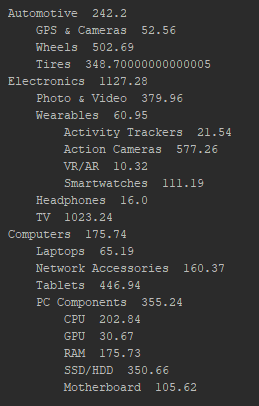
\includegraphics[width=0.5\linewidth]{1}
	\caption{Afișarea rezultatelor}
	\label{fig:1}
\end{figure}


\clearpage